
\section{Process Orchestration + API \& Webinterface}
\label{sec:process_orchestration}
\subsection{Executer Classes: Training, Infilling, Validation}


\subsection{Webinterface}

\begin{wrapfigure}[11]{r}{0.5\textwidth}
    \centering
    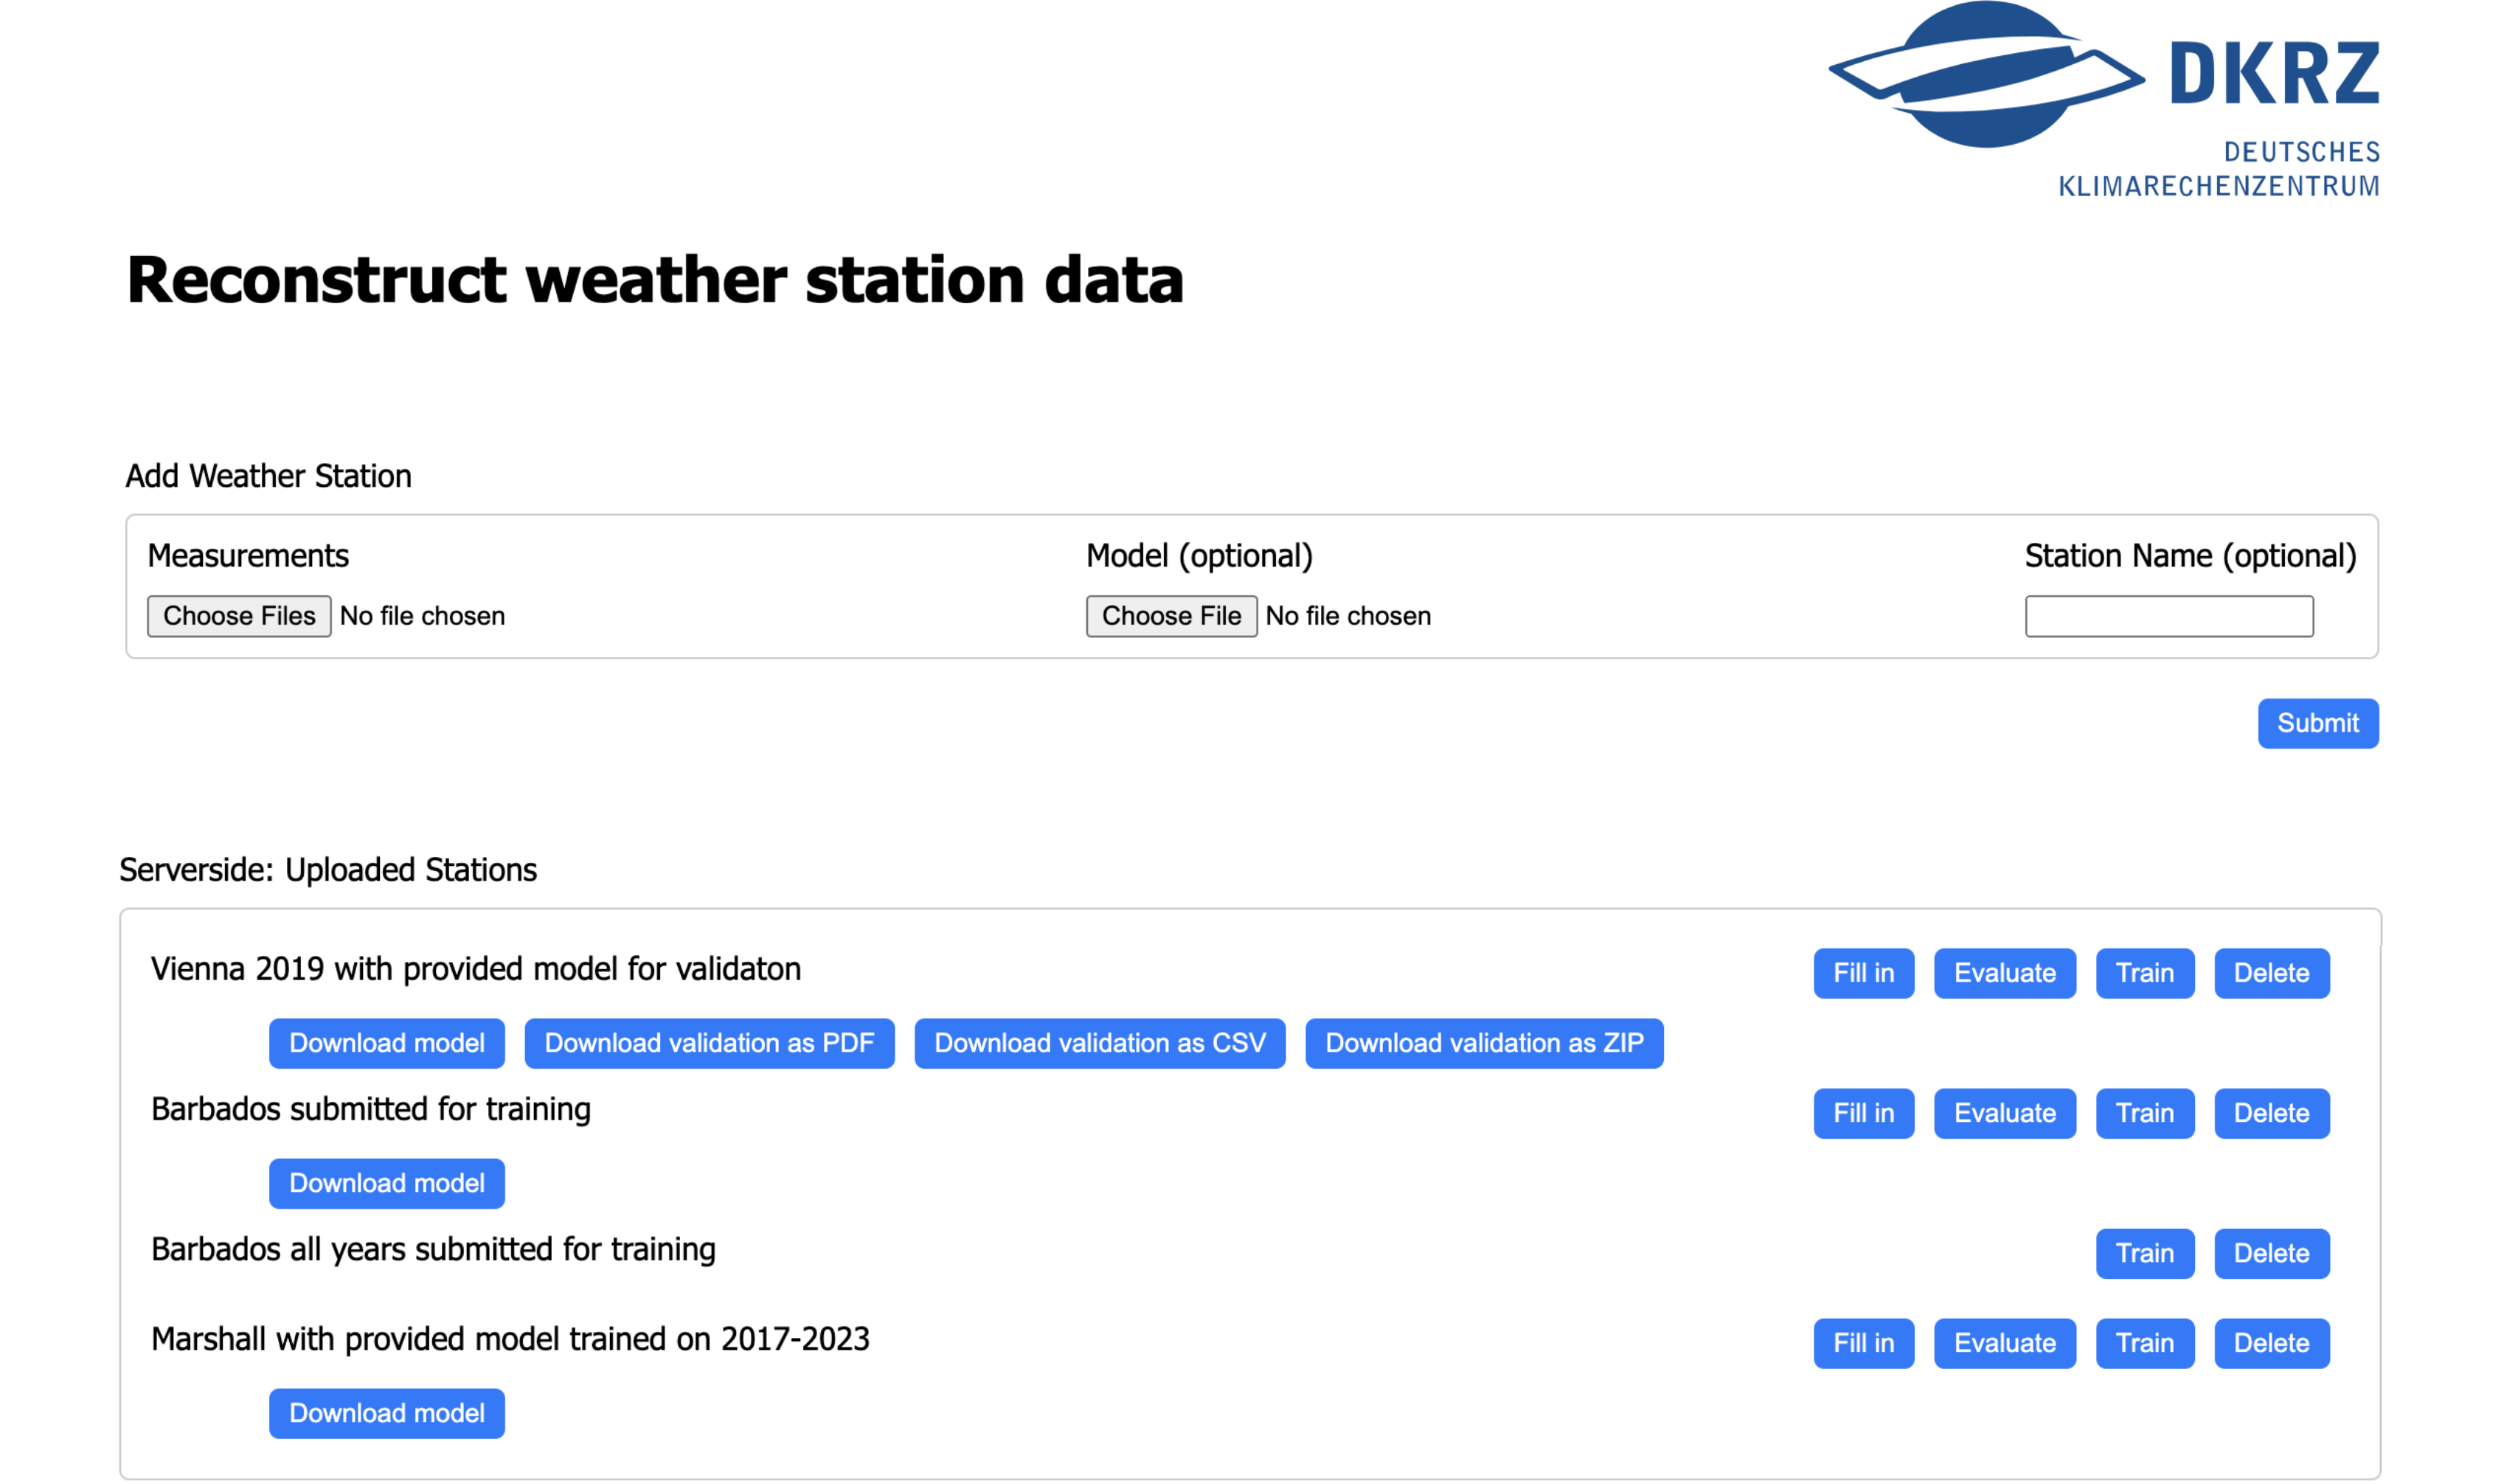
\includegraphics[width=0.5\textwidth]{resources/images/webinterface_screenshot.png}
    \caption{Screenshot of the webinterface}
    \label{fig:webinterface_screenshot}
\end{wrapfigure}

As written in the Introduction of this chapter, the benefit of establishing the abstraction layer with the executor classes, is that with minimal additional effort, API Endpoints for initiation of processes to train / validate a model as well as endpoints to retrieve the results after the processes have finished. Additionally it is possible to monitor the progress of the process through the API. The details on the API are described in \autoref{sec:api} This lays out a sufficient foundation for the implementation of a web interface, which is the main focus of this section.

The interface consists of two areas, one where the user is supposed to submit a "dataset", which in this context is meant as a collection of measurements from a weather station and the stations information such as, location, and optionally a custom name and thrid a trained model for the station that can be provided optionally as well. If no model is provided the system can train a model, and will attach it. 

The second area is a list of all datasets that the user has submitted. The API implementation allows for user identification through a unique token that is passed on to the server when the user submits a dataset, such that the user can then ask to see all datasets owned by them using that same token. The web interface automatically generates a token for the user and stores it then in the local storage of the browser, such that the user does not have to remember it.

As examples in \autoref{fig:webinterface_screenshot} show each dataset depending on its state has different options available. The deletion and train buttons they all have in common, as no model is necessary to train a model. And datasets where a model has been provided, still could be used to train a new model overwriting the old one. The "Evaluate" and "Fill in" buttons to evaluate the model over the timesteps where measurements are available, respectively to evaluate the model over the timesteps where measurements are missing.

Once a process such as training evaluation or infilling has been completed for a dataset the user can download the results anytime through the new buttons that appear in the dataset list. For example, it can be seen in \autoref{fig:webinterface_screenshot} that for the Vienna example, validation has been completed, and the user can now download a pdf with all the plots that compare the predictions with the actual measurements, or a CSV file with the same data, or a zip file that contains both and the images used in the pdf. The first Barbados example has a model attached that can be downloaded, meaning either it was provided or generated through training on the server itself. The second Barbados example has no model attached yet, meaning only the buttons "Train" and "Delete" are available, because no model was provided and no training has been done yet. 


\subsection{API Endpoints}
\label{sec:api}

% POST /data-submission
\subsubsection*{POST /data-submission}

% - GET /available-datasets/<cookie>
\subsubsection*{GET /available-datasets/<cookie>}

% - GET /train/<data-submission-id>
\subsubsection*{GET /train/<data-submission-id>}

% - GET /validate-model/<dataset-id>
\subsubsection*{GET /validate-model/<dataset-id>}

% - GET /fill-in/<dataset-id>
\subsubsection*{GET /fill-in/<dataset-id>}

% - DELETE /delete-dataset/<dataset-id>
\subsubsection*{DELETE /delete-dataset/<dataset-id>}

% - GET /download-model/<dataset-id>
\subsubsection*{GET /download-model/<dataset-id>}

% - GET /download-validation-zip/<dataset-id> (just pdf and csv available too)
\subsubsection*{GET /download-validation-zip/<dataset-id>}

% - GET /download-infilling/<dataset-id>
\subsubsection*{GET /download-infilling/<dataset-id>}
